% Copyright (C) 2014-2017 by Thomas Auzinger <thomas@auzinger.name>

\documentclass[12pt]{beamer}
\usepackage{lmodern}
\usepackage{lmodern} % Use an extension of the original Computer Modern font to minimize the use of bitmapped letters.
\usepackage{etoolbox} % true false
\usepackage[utf8]{inputenc} % Determines encoding of the input. All input files have to use UTF8 encoding.
\usepackage[T1]{fontenc}    % Determines font encoding of the output. Font packages have to be included before this line.
\usepackage{graphicx}
\usepackage{xspace}

\usepackage{qrcode}

% Extended LaTeX functionality is enables by including packages with \usepackage{...}.
\usepackage{amsmath}    % Extended typesetting of mathematical expression.
\usepackage{amssymb}    % Provides a multitude of mathematical symbols.
\usepackage{mathtools}  % Further extensions of mathematical typesetting.
\usepackage{microtype}  % Small-scale typographic enhancements.
% \usepackage[inline]{enumitem} % User control over the layout of lists (itemize, enumerate, description).
\usepackage{multirow}   % Allows table elements to span several rows.
\usepackage{booktabs}   % Improves the typesettings of tables.
\usepackage{subcaption} % Allows the use of subfigures and enables their referencing.
% \usepackage[ruled,linesnumbered]{algorithm2e} % Enables the writing of pseudo code.
% \usepackage[usenames,dvipsnames,table]{xcolor} % Allows the de\textbf{}finition and use of colors. This package has to be included before tikz.
% \usepackage{nag}       % Issues warnings when best practices in writing LaTeX documents are violated.
\usepackage[disable]{todonotes} % Provides tooltip-like todo notes.
\usepackage{hyperref}  % Enables cross linking in the electronic document version. This package has to be included second to last.
\usepackage[acronym,toc]{glossaries} % Enables the generation of glossaries and lists fo acronyms. This package has to be included last.
\usepackage{cleveref} % add page number to references (without plain)
\usepackage{nicefrac}
\usepackage[english]{babel}
\usepackage{pgfplotstable}






% Define convenience functions to use the author name and the thesis title in the PDF document properties.
\newcommand{\authorname}{\textbf{Abraham Hinteregger} \& Bernhard Haslhofer} % The author name without titles.
\newcommand{\thesistitle}{An Empirical Analysis of Monero Cross-Chain Traceability}
\setbeamertemplate{navigation symbols}{}
\usetheme{Malmoe}
\usecolortheme[]{beaver}
\useinnertheme{rectangles}
\setbeamertemplate{footline}[frame number]

% \beamersetuncovermixins{}{}


% Set PDF document properties
\hypersetup{
    pdfpagelayout   = TwoPageRight,           % How the document is shown in PDF viewers (optional).
    % linkbordercolor = {Melon},                % The color of the borders of boxes around crosslinks (optional).
    pdfauthor       = {\authorname},          % The author's name in the document properties (optional).
    pdftitle        = {\thesistitle},         % The document's title in the document properties (optional).
    pdfsubject      = {Master's Thesis Slides \authorname},              % The document's subject in the document properties (optional).
    pdfkeywords     = {cryptocurrency, linkability, traceability, heuristics, empirical} % The document's keywords in the document properties (optional).
}

% \setcounter{tocdepth}{2}% Allow only \chapter in ToC
\author{Abraham Hinteregger\inst{1,2} \and Bernhard Haslhofer\inst{1}}
% \setadvisor{Ao.Univ.Prof. Dipl.-Ing. Dr.techn.}{Günther Raidl}{}{male}
% \setfirstassistant{Dr.}{Bernhard Haslhofer}{}{male}

\title{\thesistitle}
% \subtitle{Empirical Analysis of Privacy Implications from Currency Hard-Forks}%
\institute{\inst{1} Austrian Institute of Technology \and \inst{2} Vienna University of Technology}


% Math macros
\newcommand{\figref}[1]{\figurename~\ref{#1}}
\newcommand{\TODO}[1][TODO]{\textcolor{red}{TODO}\todo{{#1}}}
\newcommand{\bigo}[1]{\ensuremath{\mathcal{O}(#1) }}
%\newtheorem{proof}{Proof}

% Name of section in reference
\newcommand{\nref}[1]{\ref{#1} \guillemotright \nameref{#1}}

% Definition imports
% !TeX root = ../CI-Thesis.tex

%% ! Helpers & Imports
\usepackage{pgfplots,pgfplotstable}
\usetikzlibrary{shapes,decorations,calc,decorations.markings, arrows.meta}
\usetikzlibrary{shapes.multipart, shapes.arrows}
\usetikzlibrary{patterns}
\usetikzlibrary{positioning,fit}
\usepgfplotslibrary{colormaps}
\usetikzlibrary{backgrounds}
%\usetikzlibrary{external}
%\tikzexternalize[prefix=external]
\pgfplotsset{colormap name=viridis}
\pgfplotsset{compat=1.16}


% from https://tex.stackexchange.com/questions/120336/adding-several-labels-year-month-to-a-graph-in-pgfplots
\usepgfplotslibrary{dateplot}
\makeatletter
\long\def\ifnodedefined#1#2#3{%
    \@ifundefined{pgf@sh@ns@#1}{#3}{#2}%
}
\makeatother



\DeclareRobustCommand{\capNode}[2][\empty]{%
\tikz[anchor=base,baseline=-.125cm]{\node[#2] (l) at (0,0) {#1};}\xspace}

\DeclareRobustCommand{\capEdge}[1]{%
\tikz[scale=0.8,anchor=base,baseline=-.125cm]{\draw[#1, -{Latex[length=1.5mm, width=1mm]}] (0,-0.25)--(0.5,0.25);}\xspace}

\DeclareRobustCommand{\capEdgePoster}[1]{%
\tikz[scale=2.25,anchor=base,baseline=0.125cm]{\draw[-{Latex[length=6mm, width=3mm]},#1] (0,0)--(0.5,0.5);}\xspace}

% Figure with source Attribution
\newcommand\sourcedFigure[2]{
\begin{tikzpicture}
	\node[] (fig) {#1};
	\node [anchor=south east,color=darkgray,inner sep=0,xshift=-15pt,yshift=0pt]at (fig.north east) {\footnotesize Source: #2};
\end{tikzpicture}}
% Figure with query Attribution
\newcommand\queryFigure[3]{
\begin{tikzpicture}
	\node[] (fig) {#1};
	\node [anchor=south east,color=darkgray,inner sep=0,xshift=-15pt,yshift=0pt]at (fig.north east) {\footnotesize SQL: \url{#2}, CSV: \url{#3}};
\end{tikzpicture}}

% Global Color definitions
  
\definecolor{vir0}{rgb}{0.267004, 0.004874, 0.329415}
\definecolor{vir1}{rgb}{0.282623, 0.140926, 0.457517}
\definecolor{vir2}{rgb}{0.253935, 0.265254, 0.529983}
\definecolor{vir3}{rgb}{0.206756, 0.371758, 0.553117}
\definecolor{vir4}{rgb}{0.163625, 0.471133, 0.558148}
\definecolor{vir5}{rgb}{0.127568, 0.566949, 0.550556}
\definecolor{vir6}{rgb}{0.134692, 0.658636, 0.517649}
\definecolor{vir7}{rgb}{0.266941, 0.748751, 0.440573}
\definecolor{vir8}{rgb}{0.477504, 0.821444, 0.318195}
\definecolor{vir9}{rgb}{0.741388, 0.873449, 0.149561}
\definecolor{vir10}{rgb}{0.993248, 0.906157, 0.143936}

\pgfplotsset{
	xmaxCutoff/.style={xmax = 2018-08-15},
	fancyDateTicks/.style={
		, date coordinates in=x
		, xmin = 2014-03-15
		, xmaxCutoff % , xmax = 2018-08-15
		, xtick=data
		, extra x ticks={2014-08-01,2015-06-15,2016-06-15,2017-06-15,2018-03-15} % where year ticks should be placed
		, extra x tick style={
			, yshift=-3ex
			, tick label style={rotate=-90}
			, xticklabel=\year
			, xticklabel style={name={}}
			, major tick length=0pt
			}
			, xticklabel style={
				, rotate = 90
				, font=\scriptsize
			, anchor=near xticklabel
			, name=\ifnodedefined{start\year} % Have we already started this year?
			{end\year}  % Then this could be the last month
			{start\year} % Otherwise, start the year
			, append after command=
			\pgfextra{\pgfmathtruncatemacro\lastyear{\year-1}}
			\ifnodedefined{end\lastyear}
			{{\ifnum\month=1 (start\lastyear.165) edge (end\lastyear.195) \pgfextra{\xdef\finalyear{\year}}\fi}}{}
			}
			, after end axis/.code={\draw (start\finalyear.165) -- (end\finalyear.195);}
			, xticklabel=\month
			, date ZERO=2014-04-01,% <- improves precision!
	},
	fancyDateTicksSlides/.style={
		, date coordinates in=x
		, xmin = 2014-03-15
		, xmaxCutoff % , xmax = 2018-08-15
		, xtick=data
		, extra x ticks={2014-08-01,2015-06-15,2016-06-15,2017-06-15,2018-04-15} % where year ticks should be placed
		, extra x tick style={
			% , yshift=-3ex
			, tick label style={rotate=-90}
			, xticklabel=\year
			, xticklabel style={name={}}
			, major tick length=0pt
			}
			, xticklabel style={
				, rotate = 90
				, font=\scriptsize
				% , scale=0.5
				, anchor=near xticklabel
				, name=\ifnodedefined{start\year}{end\year}{start\year}
				% , append after command=\pgfextra{\pgfmathtruncatemacro\lastyear{\year-1}}
			% \ifnodedefined{end\lastyear}
			% {{\ifnum\month=1 (start\lastyear.165) edge (end\lastyear.195) \pgfextra{\xdef\finalyear{\year}}\fi}}{}
			}
			% , after end axis/.code={\draw (start\finalyear.165) -- (end\finalyear.195);}
			, xticklabel=\empty
			, date ZERO=2014-04-01,% <- improves precision!
	}
}

\tikzset{
	niceNums/.style = {
		,	/pgf/number format/fixed
		,	/pgf/number format/1000 sep=\thinspace
	},
	twoColorDashed/.style 2 args={
		draw
		,very thick
		,smooth
		,tension=0.2
		,#2
	,postaction={draw
		,ultra thick
		,densely dashed
		,#1
	}},
	virNode/.style={
		% pgfplots/colormap name=viridis,
		color of colormap={#1 * 1000-1}, % offset * 2 + scale <= 2000
		draw=.!60!black,
		fill=.!70!white,
		text = black
	},
	virNodeDark/.style={
		% pgfplots/colormap name=viridis,
		color of colormap={#1 * 1000-1}, % offset * 2 + scale <= 2000
		draw=.!70!black,
		fill=.!90!white,
		text = black
	},
	nodeWhite/.style={
		draw=white!40!black,
		fill=black!30!white,
		text = black
	},
	nodeBlack/.style={
		draw=black!40!black,
		fill=black!50!white,
		text = white
	},
	waterFall/.style={
		% pgfplots/colormap name=viridis,
		color of colormap={#1 * 99 - 50}, 
		draw=.!60!black,
		fill=.!70!white,
		text = black
	},	
	txColor/.style={
		color of colormap={400},
		draw=.!70!black,
		fill=.!90!white,
		text = black
	},
	txColorLight/.style={
		color of colormap={400},
		draw=.!70!black,
		fill=.!90!black,
		text = white
	},
	txSpentColor/.style={
		color of colormap={600},
		draw=.!70!black,
		fill=.!80!white,
		text = black
	},
	XMRColor/.style={
		color of colormap={850},
		draw=.!70!black,
		fill=.!80!black,
		text = black
	},
	XMOColor/.style={
		color of colormap={400},
		draw=.!80!black,
		fill=.!90!white,
		text = white
	},
	XMVColor/.style={
		color of colormap={100},
		draw=.!80!black,
		fill=.!80!white,
		text = white
	},
	blockColor/.style={
		color of colormap={850},
		draw=.!70!black,
		fill=.!80!black,
		text = black
	},
	blockDarkColor/.style={
		color of colormap={850},
		draw=.!70!black,
		fill=.!100!white,
		text = black
	},
}


% Consistent shapes for same structures
\tikzset{
	TX/.style={
		,	rounded corners = 0.25mm
		,	thick
		,	txColor
	},
	TXs/.style={
		,	rounded corners = 0.25mm
		,	thick
		,	txSpentColor
	},
	Block/.style={
		,	very thick
		,	rounded corners = 0.5mm
		,	blockColor
	},
	BlockD/.style={
		,	rounded corners = 0.5mm
		,	blockDarkColor
		,	inner sep = 0.75mm
	},
	outIndex/.style={
		,	rounded corners = 0.3mm
		,	blockColor
		,	inner sep = 0.3mm
		,	draw=none
	}
} 

% Plot cycle list
%! Unused & invalid values
\pgfplotscreateplotcyclelist{connCountList}{
	{bankCount=6},
	{bankCount=5},
	{bankCount=4},
	{bankCount=3},
	{bankCount=2},
	{bankCount=1},
	{bankCount=0},
}


% put figures on top of pages  
\makeatletter
\setlength{\@fptop}{8pt}
\makeatother


% Reference plotlines in text
\newcommand{\plotref}[1]{{[\,\ref{#1}\,]}\xspace}

%	This file was generated by /python/data_table.py. Definitions etc. can be found there.
%	 Blockchain meta data
\def\XMRDATEF{2014-04-18\xspace}
\def\XMODATEF{2018-04-06\xspace}
\def\XMVDATEF{2018-05-03\xspace}
\def\XMRDATEL{2018-08-31\xspace}
\def\XMODATEL{2018-08-31\xspace}
\def\XMVDATEL{2018-08-31\xspace}
\def\XMOFORK{1\,546\,599\xspace}
\def\XMVFORK{1\,564\,965\xspace}
\def\XMRFIRST{1\xspace}
\def\XMOFIRST{1\,546\,600\xspace}
\def\XMVFIRST{1\,564\,966\xspace}
%	 Height at analysis cutoff
\def\XMRHEIGHT{1\,651\,346\xspace}
\def\XMRHEIGHTo{1\,651\,346\xspace}
\def\XMRHEIGHTv{1\,651\,346\xspace}
\def\XMOHEIGHT{1\,651\,728\xspace}
\def\XMVHEIGHT{1\,647\,778\xspace}
%	 Last block timestamp before cutoff date
\def\XMRTIMESTAMP{2018-08-31 23:58:15\xspace}
\def\XMOTIMESTAMP{2018-08-31 23:59:45\xspace}
\def\XMVTIMESTAMP{2018-08-31 23:46:43\xspace}
%	 Number of TXs
\def\XMRTX{4\,955\,908\xspace}
\def\XMRTXo{771\,287\xspace}
\def\XMRTXv{603\,413\xspace}
\def\XMOTX{146\,475\xspace}
\def\XMVTX{146\,215\xspace}
%	 Number of Coinbase TXs
\def\XMRCB{1\,651\,347\xspace}
\def\XMRCBo{104\,747\xspace}
\def\XMRCBv{86\,381\xspace}
\def\XMOCB{105\,729\xspace}
\def\XMVCB{82\,814\xspace}
%	 Number of Outputs
\def\XMRTXOUT{28\,878\,846\xspace}
\def\XMRTXOUTo{1\,859\,970\xspace}
\def\XMRTXOUTv{1\,456\,810\xspace}
\def\XMOTXOUT{198\,618\xspace}
\def\XMVTXOUT{450\,773\xspace}
%	 Number of Inputs (Rings)
\def\XMRR{24\,760\,168\xspace}
\def\XMRRo{1\,528\,763\xspace}
\def\XMRRv{1\,182\,727\xspace}
\def\XMOR{244\,965\xspace}
\def\XMVR{212\,919\xspace}
%	 Number of nontrivial rings
\def\XMRRNT{12\,538\,632\xspace}
\def\XMRRNTo{1\,516\,342\xspace}
\def\XMRRNTv{1\,175\,486\xspace}
\def\XMORNT{241\,464\xspace}
\def\XMVRNT{212\,919\xspace}
%	 Number of traced nontrivial rings
\def\XMRRNTL{4\,212\,422\xspace}
\def\XMRRNTLo{56\,456\xspace}
\def\XMRRNTLv{27\,844\xspace}
\def\XMORNTL{50\,861\xspace}
\def\XMVRNTL{7\,671\xspace}
%	 Number of ring members
\def\XMRRM{70\,767\,723\xspace}
\def\XMRRMo{11\,563\,837\xspace}
\def\XMRRMv{9\,014\,131\xspace}
\def\XMORM{1\,243\,479\xspace}
\def\XMVRM{1\,701\,036\xspace}
%	 Number of identified mixins
\def\XMRIM{16\,270\,257\xspace}
\def\XMRIMo{497\,570\xspace}
\def\XMRIMv{295\,107\xspace}
\def\XMOIM{230\,128\xspace}
\def\XMVIM{49\,035\xspace}
%	 Number of identified reals
\def\XMRIR{16\,433\,958\xspace}
\def\XMRIRo{68\,877\xspace}
\def\XMRIRv{35\,085\xspace}
\def\XMOIR{54\,362\xspace}
\def\XMVIR{7\,671\xspace}
%	 Some Monerov Metadata
\def\XMVPUBLICBLOCK{1\,565\,244\xspace}
\def\XMVPUBLICDATE{2\,005\xspace}
%	 Recent XMR data
\def\recenta{2018-04-01\xspace}
\def\recentb{2018-08-31\xspace}
\def\recentnofork{25\,256\xspace}
\def\recentfork{73\,321\xspace}
\def\recentmixinnofork{203\,251\xspace}
\def\recentmixinfork{544\,131\xspace}
\def\recenttotal{617\,452\xspace}
\def\recentrm{11\,826\,525\xspace}
\def\recenttotalnf{228\,507\xspace}
\def\recentrings{1\,565\,858\xspace}
\def\recenttxnoncb{685\,608\xspace}
%	 Spent inputs
\def\numspent{13\,240\xspace}
%	 Shared keyimgs
\def\sharedxmo{56\,663\xspace}
\def\sharedxmv{6\,734\xspace}
%   Redeem stats
\def\XMOREDEEM{50\,273\xspace}
\def\XMVREDEEM{5\,506\xspace}
\def\XMOREDEEMCORR{6\,497\xspace}
\def\XMVREDEEMCORR{1\,231\xspace}


% \usepgfplotslibrary{external}
% \tikzexternalize%[prefix=precompiled/]
\makeatletter
\let\@@magyar@captionfix\relax
\makeatother

\newcommand{\backupbegin}{
   \newcounter{finalframe}
   \setcounter{finalframe}{\value{framenumber}}
}
\newcommand{\backupend}{
   \setcounter{framenumber}{\value{finalframe}}
}

\begin{document}
\selectlanguage{english}
% \date{November 13$^\text{th}$, 2018}
\maketitle
% !TeX root = ../CI-Slides.tex
% \tableofcontents
% ---------------------------------------------------------%

\section{Introduction}
\subsection{Cryptocurrencies}
\begin{frame}{Cryptocurrencies}
	\begin{itemize}
	\item \cite{nakamoto_bitcoin:_2008}	laid the foundation of modern cryptocurrencies (scheme for trusted decentralized transactions)	
	\item Transactions have inputs (references to previous outputs) and outputs
	\item Each output is issued to address of a user (public key)
	\item Recipient can spend outputs with private key
	\end{itemize}
\end{frame}

\begin{frame}{Blockchain}
	\resizebox{\textwidth}{!}{% !TeX root = ../CI-Thesis.tex
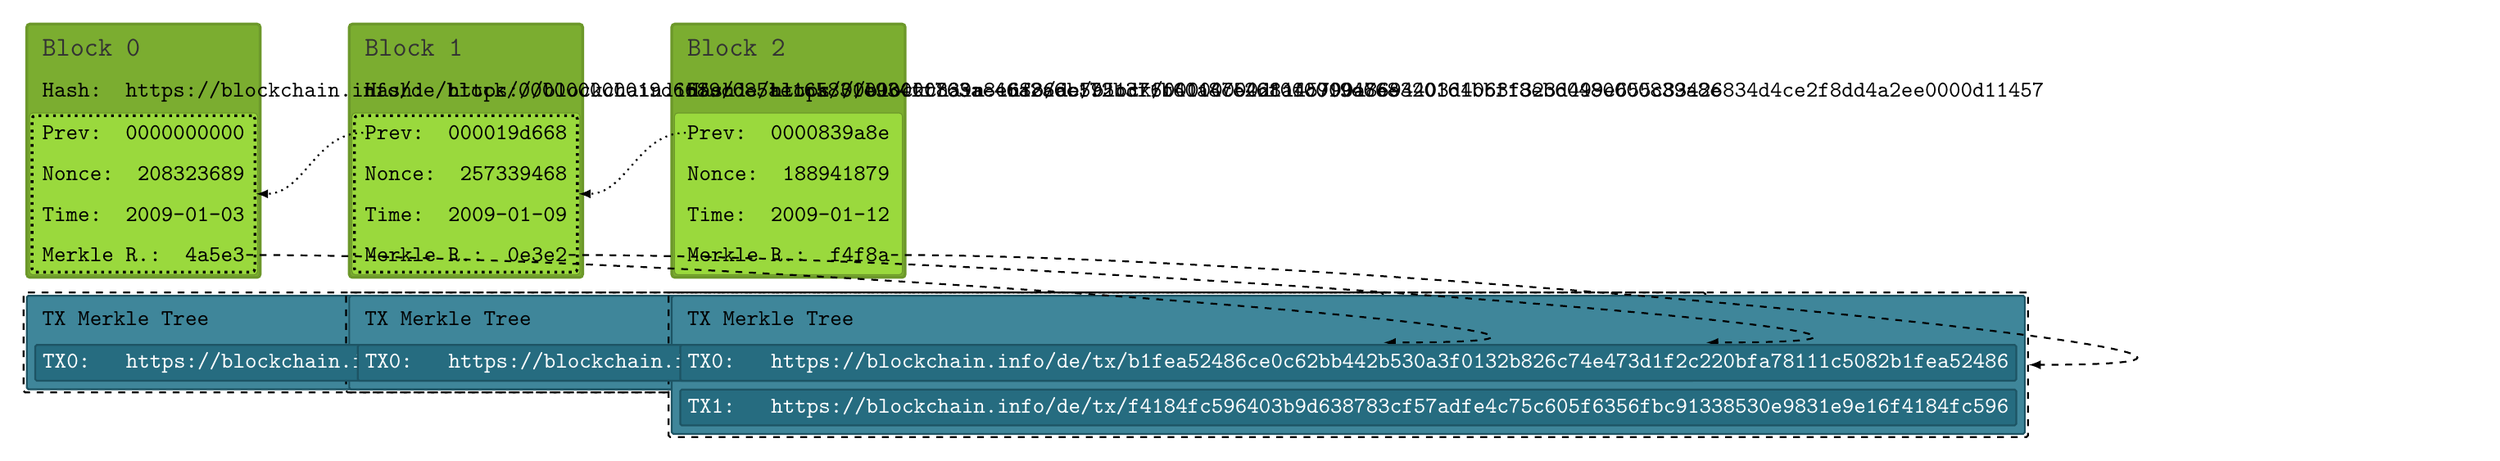
\begin{tikzpicture}[
	,	scale=1.0
	,	node distance=4mm,
	,	font=\ttfamily,
	,	BlockTitle/.style={font=\fontsize{12}{12}\color{black!80}\ttfamily}
	,	TXHeader/.style={below=of T.west,anchor=north west, yshift = -3.5mm}
] 
\def\dist{5}

\node[BlockTitle] (Bt) at ($(\dist*0,0)$) {Block 0 };
\node[below=of Bt.west,anchor=north west] (Hash0) {Hash: \href{https://blockchain.info/de/block/000000000019d6689c085ae165831e934ff763ae46a2a6c172b3f1b60a8ce26f}{000019d668}};
\node[below=of Hash0.west,anchor=north west] (Prev0) {Prev: 0000000000};
\node[below=of Prev0.west,anchor=north west] (T) { Nonce: 208323689};
%\node[TX, below=of T.west,anchor=north west,opacity=0] (T) { TX1: \ 0af121280a };
\node[below=of T.west,anchor=north west] (T) { Time: 2009-01-03};
\node[below=of T.west,anchor=north west] (T) { Merkle R.: 4a5e3};


\node[TXHeader] (TXt) {TX Merkle Tree};

\node[TX,txColorLight, below=of TXt.west,anchor=north west] (TXs) { TX0: \ \href{https://blockchain.info/de/tx/4a5e1e4baab89f3a32518a88c31bc87f618f76673e2cc77ab2127b7afdeda33b}{4a5e321e4b}};

\begin{scope}[on background layer]
	\node[Block,fit={(Bt) (T)}] (B1) {};
	\node[BlockD,fit={(Prev0) (T)}] (B1h) {};
	\node[BlockD,draw=black, fill=none, inner sep = 1pt, very thick, dotted, fit={(Prev0) (T)}] (B1H) {};
	\node[TX,fit={(TXt)(TXs)}] (TXb2) {};
	\node[TX, draw=black, fill=none, thick, inner sep = 1pt, dashed, fit={(TXb2)}] (MRH) {};
\end{scope}
\path[thick, dashed, black,-latex]($(T.east)-(0.1,0)$) edge[out = 0, in = 0] (MRH.east);

\node[BlockTitle] (Bt) at ($(\dist*1,0)$) {Block 1 };
\node[below=of Bt.west,anchor=north west] (Hash1) {Hash: \href{https://blockchain.info/de/block/00000000839a8e6886ab5951d76f411475428afc90947ee320161bbf18eb6048}{0000839a8e}};
\node[below=of Hash1.west,anchor=north west] (Prev1) {Prev: 000019d668};
\node[below=of Prev1.west,anchor=north west] (T) { Nonce: 257339468};
%\node[TX, below=of T.west,anchor=north west] (T) { TX1: \ 0ab112023a };
\node[below=of T.west,anchor=north west] (T) { Time: 2009-01-09 };
\node[below=of T.west,anchor=north west] (T) { Merkle R.: 0e3e2};


\node[TXHeader] (TXt) {TX Merkle Tree};
\node[TX,txColorLight, below=of TXt.west,anchor=north west] (TXs) { TX0: \ \href{https://blockchain.info/de/tx/0e3e2357e806b6cdb1f70b54c3a3a17b6714ee1f0e68bebb44a74b1efd512098}{0e3e2357e8}};

\begin{scope}[on background layer]
	\node[Block,fit={(Bt) (T)}] (B1) {};
	\node[BlockD,fit={(Prev1) (T)}] (B1h) {};
	\path[thick, dashed, black,-latex, dotted]($(Prev1.west)+(0.1,0)$) edge[out=180, in = 0] (B1H.east);
	\node[BlockD,draw=black, fill=none, inner sep = 1pt, very thick, dotted, fit={(Prev1) (T)}] (B1H) {};
	\node[TX,fit={(TXt)(TXs)}] (TXb2) {};
	\node[TX, draw=black, fill=none, thick, inner sep = 1pt, dashed, fit={(TXb2)}] (MRH) {};
\end{scope}
\path[thick, dashed, black,-latex]($(T.east)-(0.1,0)$) edge[out = 0, in = 0] (MRH.east);

% \draw[ultra thick,-latex] (Prev1.west)--(Hash0.east);

\node[BlockTitle] (Bt) at ($(\dist*2,0)$) {Block 2 };
\node[below=of Bt.west,anchor=north west] (Hash2) {Hash: \href{https://blockchain.info/de/block/00000000d1145790a8694403d4063f323d499e655c83426834d4ce2f8dd4a2ee}{0000d11457}};
\node[below=of Hash2.west,anchor=north west] (Prev2) {Prev: 0000839a8e};
\node[below=of Prev2.west,anchor=north west] (T) { Nonce: 188941879};
\node[below=of T.west,anchor=north west] (T) { Time:  2009-01-12 };
\node[below=of T.west,anchor=north west] (T) { Merkle R.: f4f8a};


\node[TXHeader] (TXt) {TX Merkle Tree};
\node[TX,txColorLight, below=of TXt.west,anchor=north west] (TXs) { TX0: \ \href{https://blockchain.info/de/tx/b1fea52486ce0c62bb442b530a3f0132b826c74e473d1f2c220bfa78111c5082}{b1fea52486}};
\node[TX,txColorLight, below=of TXs.west,anchor=north west] (TXs) { TX1: \ \href{https://blockchain.info/de/tx/f4184fc596403b9d638783cf57adfe4c75c605f6356fbc91338530e9831e9e16}{f4184fc596}};

\begin{scope}[on background layer]
	\node[Block,fit={(Bt) (T)}] (B1) {};
	\node[BlockD,fit={(Prev2) (T)}] (B1h) {};
	\path[thick, dashed, black,-latex, dotted]($(Prev2.west)+(0.1,0)$) edge[out=180, in = 0] (B1H.east);
	\node[TX,fit={(TXt)(TXs)}] (TXb2) {};
	\node[TX, draw=black, fill=none, thick, inner sep = 1pt, dashed, fit={(TXb2)}] (MRH) {};
\end{scope}
\path[thick, dashed, black,-latex]($(T.east)-(0.1,0)$) edge[out = 0, in = 0] (MRH.east);

% \draw[ultra thick,-latex] (Prev2.west)--(Hash1.east);

\end{tikzpicture} }
\end{frame}

\begin{frame}{Transaction}
	\resizebox{\textwidth}{!}{% !TeX root = ../CI-Thesis.tex
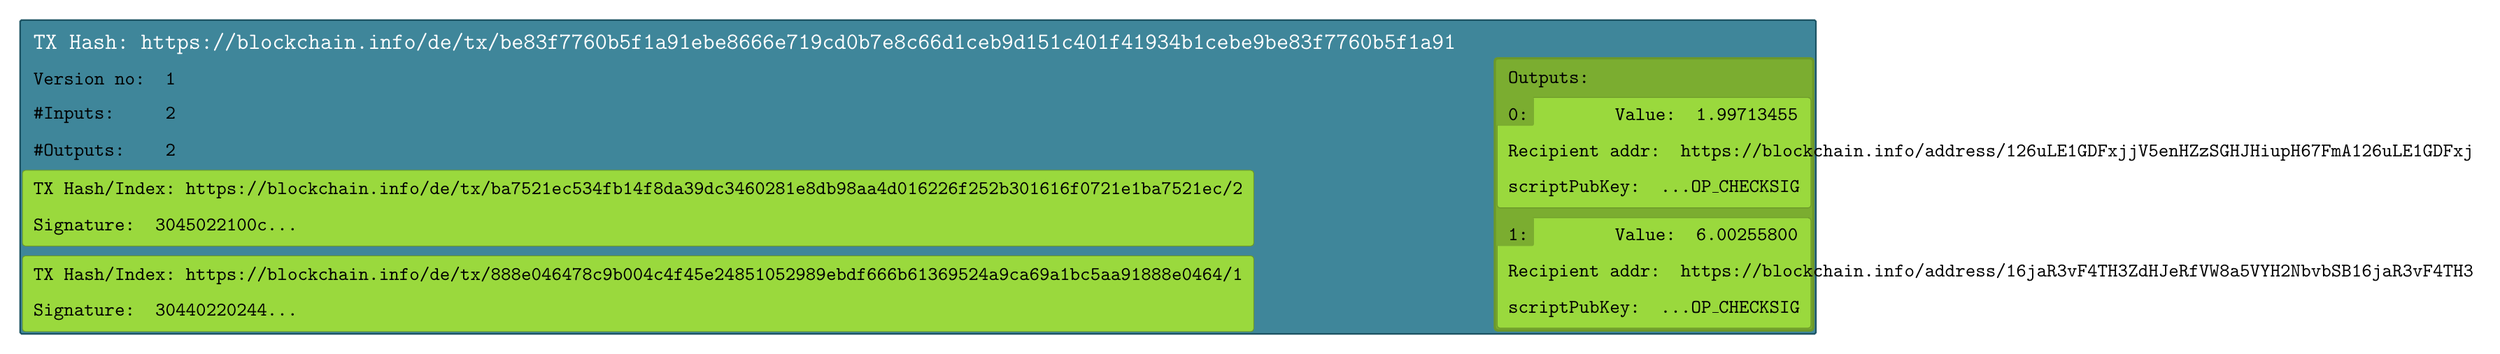
\begin{tikzpicture}[
	,	scale=1.0
	,	node distance=4mm,
	,	font=\ttfamily\bfseries,
	,	BlockTitle/.style={font=\fontsize{12}{12}\color{black!80}\ttfamily\bfseries}
	,	TxTitle/.style={font=\fontsize{12}{12}\color{white}\ttfamily\bfseries}
	,	-latex
] 
\def\dist{6}

% https://webbtc.com/tx/a1075db55d416d3ca199f55b6084e2115b9345e16c5cf302fc80e9d5fbf5d48d.json

\node[TxTitle] (BT) at ($(\dist*0,0)$) {TX Hash:\ \href{https://blockchain.info/de/tx/be83f7760b5f1a91ebe8666e719cd0b7e8c66d1ceb9d151c401f41934b1cebe9}{be83f7760b5f1a91}};
\node[below=of BT.west,anchor=north west] (Hash0) {Version no:\quad1};
\node[below=of Hash0.west,anchor=north west] (Hash0) {\#Inputs:\qquad\ 2};
\node[below=of Hash0.west,anchor=north west] (numOut) {\#Outputs:\quad\ \ 2};

\node[below=of numOut.west,anchor=north west] (H1) {TX Hash/Index:\ \href{https://blockchain.info/de/tx/ba7521ec534fb14f8da39dc3460281e8db98aa4d016226f252b301616f0721e1}{ba7521ec}/2};
\node[below=of H1.west,anchor=north west] (Sig1) {Signature: 3045022100c\ldots};

\node[below=of Sig1.west,anchor=north west, yshift=-2mm] (H2) {TX Hash/Index:\ \href{https://blockchain.info/de/tx/888e046478c9b004c4f45e24851052989ebdf666b61369524a9ca69a1bc5aa91}{888e0464}/1};
\node[below=of H2.west,anchor=north west] (Sig2) {Signature: 30440220244\ldots};


\node[right=of BT.south east,anchor=north west,yshift=-0.6mm, xshift=3mm] (Outs) {Outputs:};
\node[below=of Outs.west,anchor=north west] (i1) {0:};
\node[right=of i1.north east,anchor=north west] (O1) {\ \ \ \ \ Value: 1.99713455};
\node[below=of i1.west,anchor=north west] (O1) {Recipient addr: \href{https://blockchain.info/address/126uLE1GDFxjjV5enHZzSGHJHiupH67FmA}{126uLE1GDFxj}};
\node[below=of O1.west,anchor=north west] (O1) {scriptPubKey: \ldots{}OP\_CHECKSIG};
\node[below=of O1.west,anchor=north west, yshift=-2mm] (i2) {1:};
\node[right=of i2.north east,anchor=north west] (O2) {\ \ \ \ \ Value: 6.00255800};
\node[below=of i2.west,anchor=north west] (O2) {Recipient addr:  \href{https://blockchain.info/address/16jaR3vF4TH3ZdHJeRfVW8a5VYH2NbvbSB}{16jaR3vF4TH3}};
\node[below=of O2.west,anchor=north west] (O2) {scriptPubKey: \ldots{}OP\_CHECKSIG};

\node[opacity=0, right=of O2.east, xshift=-6mm, yshift=-2mm](Stretch){ };
\begin{scope}[on background layer]
	\node[TX,fit={(BT) (Sig2) (Stretch)}] (B1) {};
	\node[BlockD,fit={(H1) (Sig1)}] (B1h) {};
	\node[BlockD,fit={(H2) (Sig2)}] (B1h) {};
	\node[Block,fit={(Outs) (O2)}] (B1h) {};

	\node[BlockD,fit={(i1) (O1)}] (B1h) {};
	\node[BlockD,fit={(i2) (O2)}] (B1h) {};

	\node[outIndex, fit={(i1)}, xshift=-0.55mm, yshift=0.55mm] (B1h) {};
	\node[outIndex, fit={(i2)}, xshift=-0.55mm, yshift=0.55mm] (B1h) {};
\end{scope}

\end{tikzpicture} }
\end{frame}

\subsection{Monero}
\begin{frame}{Monero}\label{sec:monero}
	\begin{itemize}
		\item Public nature of Bitcoin TX history prevents meaningful level of anonymity
		\item Monero (based on CryptoNote, \cite{van_saberhagen_cryptonote_2013}) addresses this issue with the following methods:
		\begin{itemize}[<+-|alert@+>]
			\item Stealth Addresses (hide recipient addr.) $\to$ unlinkability (p.~\ref{sec:mih})
			\item \alert<4->{Ring Signatures (obfuscate spent outputs) $\to$ untraceability}
			\item Confidential Transactions (hide amounts) $\to$ fungibility
		\end{itemize} 
	\end{itemize}
\end{frame}

\subsection{Ring Signatures}
\begin{frame}{Ring Signatures \& Traceability}
	\vspace*{-10pt}
	\begin{itemize}[<+->]
		\item Each TX input references:
		\begin{itemize}
			\item Bitcoin: Output from older TX (TXO)
			\item Monero: Non-empty set of TXOs (a ring)
		\end{itemize}
		\item One ringmember is real, the others are decoys (mixins)
		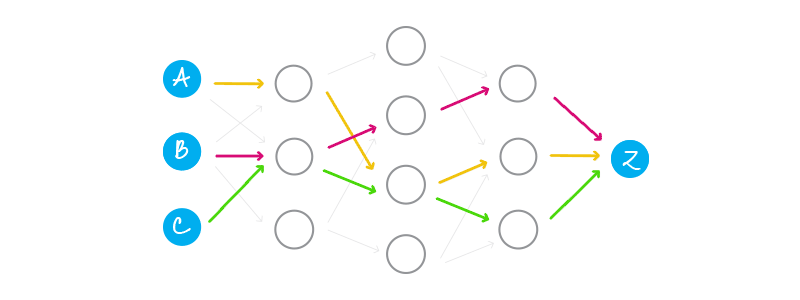
\includegraphics[width=\textwidth]{./img/slides/cn-44.png}
{		\hspace*{90pt}\scriptsize Source: \url{https://cryptonote.org/inside/}}
		\item Decoys are sampled from set of eligible outputs
	\end{itemize}
\end{frame}
\section{Traceability Analysis}


\subsection{Traceability Methods I (ZMR \& IR)}
\begin{frame}{Zero Mixin Removal \& Intersection Removal}
	\resizebox{\textwidth}{!}{% !TeX root = ../../CI-Slides.tex
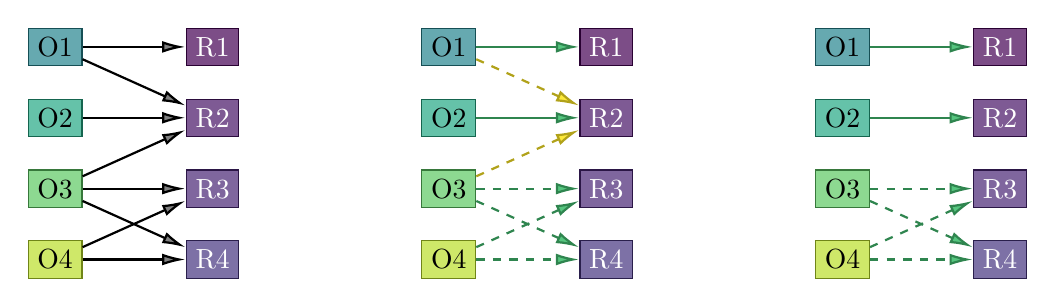
\begin{tikzpicture}[scale=1.0, -{Latex[length=3mm, width=1.5mm]}
    ,    remEdge/.style={thick, dashed, virNodeDark=1.0} 
    ,    sureEdge/.style={thick, virNodeDark=0.7} 
    ,    spentEdge/.style={thick, dashed, virNodeDark=0.7}] 
\coordinate (C1) at (2,2);

\begin{scope}[xshift=-5.0cm]
    \node[virNode=0.45] (X1) at (-1,0.9){O1}; 
    \node[virNode=0.60] (X2) at (-1,0){O2}; 
    \node[virNode=0.75] (X3) at (-1,-0.9){O3}; 
    \node[virNode=0.90] (X4) at (-1,-0.9*2){O4}; 
    \node[virNode=0.0,text=white] (Y1) at (1,0.9){R1};
    \node[virNode=0.05,text=white] (Y2) at (1,0){R2};
    \node[virNode=0.1,text=white] (Y3) at (1,-0.9){R3};
    \node[virNode=0.15,text=white] (Y4) at (1,-0.9*2){R4};
   
    \path[thick, nodeBlack](X1) edge[] (Y1);
    \path[thick, nodeBlack](X1) edge[] (Y2);
    \path[thick, nodeBlack](X2) edge[] (Y2);
    \path[thick, nodeBlack](X3) edge[] (Y2);
    \path[thick, nodeBlack](X3) edge[] (Y3);
    \path[thick, nodeBlack](X3) edge[] (Y4);
    \path[thick, nodeBlack](X4) edge[] (Y3);
    \path[thick, nodeBlack](X4) edge[] (Y4);
\end{scope}
\uncover<2->{
\begin{scope}[xshift=0.0cm]
    \node[virNode=0.45] (X1) at (-1,0.9){O1}; 
    \node[virNode=0.60] (X2) at (-1,0){O2}; 
    \node[virNode=0.75] (X3) at (-1,-0.9){O3}; 
    \node[virNode=0.90] (X4) at (-1,-0.9*2){O4}; 
    \node[virNode=0.0,text=white] (Y1) at (1,0.9){R1};
    \node[virNode=0.05,text=white] (Y2) at (1,0){R2};
    \node[virNode=0.1,text=white] (Y3) at (1,-0.9){R3};
    \node[virNode=0.15,text=white] (Y4) at (1,-0.9*2){R4};
    
    \path[sureEdge](X1) edge[] (Y1);
\uncover<4->{
    \path[remEdge](X1) edge[] (Y2);
    \path[remEdge](X3) edge[] (Y2);
}
\uncover<5->{
    \path[sureEdge](X2) edge[] (Y2);
}
\uncover<3->{
    \path[spentEdge](X3) edge[] (Y3);
    \path[spentEdge](X3) edge[] (Y4);
    \path[spentEdge](X4) edge[] (Y3);
    \path[spentEdge](X4) edge[] (Y4);
}
\end{scope}
}
\uncover<5->{
\begin{scope}[xshift=5.0cm]
    \node[virNode=0.45] (X1) at (-1,0.9){O1}; 
    \node[virNode=0.60] (X2) at (-1,0){O2}; 
    \node[virNode=0.75] (X3) at (-1,-0.9){O3}; 
    \node[virNode=0.90] (X4) at (-1,-0.9*2){O4}; 
    \node[virNode=0.0,text=white] (Y1) at (1,0.9){R1};
    \node[virNode=0.05,text=white] (Y2) at (1,0){R2};
    \node[virNode=0.1,text=white] (Y3) at (1,-0.9){R3};
    \node[virNode=0.15,text=white] (Y4) at (1,-0.9*2){R4};

    \path[sureEdge](X1) edge[] (Y1);
    \path[sureEdge](X2) edge[] (Y2);
    \path[spentEdge](X3) edge[] (Y3);
    \path[spentEdge](X3) edge[] (Y4);
    \path[spentEdge](X4) edge[] (Y3);
    \path[spentEdge](X4) edge[] (Y4);
\end{scope}
}
\end{tikzpicture} }
	\begin{itemize}
		\item Outputs O1-O4 are referenced in rings R1-R4
		\item<2-> R1 only references O1 $\implies$ must be the real input
		\item<3-> $I = \{R3,R4\}$ reference $O=\{O3,O4\}$  \\
		\qquad	$|I| = |O|$ $\implies$ O3 \& O4 spent in R3 \& R4
		\item<4-> $R2$ only has one non-mixin reference remaining.
	\end{itemize}
\end{frame}

\begin{frame}{Output Merging Heuristic (OMH)}
	\begin{itemize}
		\item Output merging mostly due to denomination splitting:
		\begin{itemize}
			\item Initially, amounts were disclosed on blockchain
			\item Ring signatures required multiple outputs with identical amounts
			\item Outputs were partitioned to facilitate this (7 $\to$ 5 + 2)
		\end{itemize}
	\end{itemize}
	\uncover<2->{
	\resizebox{\textwidth}{!}{% !TeX root = ../../CI-Slides.tex
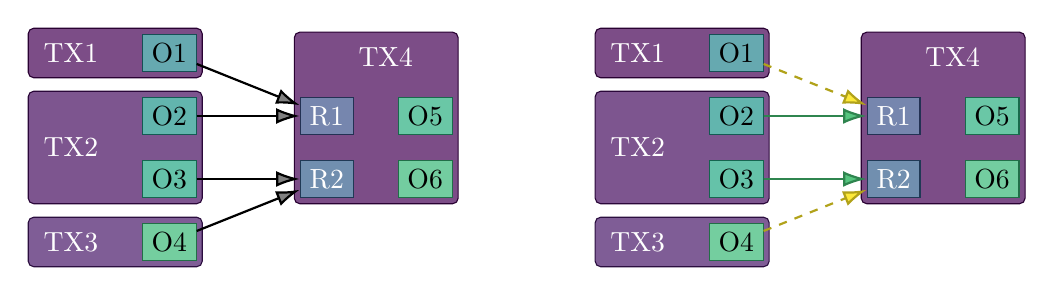
\begin{tikzpicture}[scale=1.0, -{Latex[length=3mm, width=2mm]}
    ,   remEdge/.style={thick, dashed, virNodeDark=1.0} 
    ,   txNode/.style={opacity=1.0,inner sep=2pt,rounded corners=2pt}
    ,   sureEdge/.style={thick, virNodeDark=0.7}] 
\coordinate (C1) at (2,2);


\begin{scope}[xshift=-3.6cm]
    \node[text=white] (TX2) at (-2.25,0.8){TX1};
    \node[virNode=0.450] (X3) at (-1,0.8){O1}; 

    \node[text=white] (TX1) at (-2.25,-0.4){TX2};
    \node[virNode=0.525] (X1) at (-1,0){O2}; 
    \node[virNode=0.600] (X2) at (-1,-0.8){O3}; 
    
    \node[text=white] (TX3) at (-2.25,-1.6){TX3};
    \node[virNode=0.675] (X4) at (-1,-1.6){O4}; 
    \node[virNode=0.25,text=white] (Y1) at (1,0){R1};
    \node[virNode=0.30,text=white] (Y2) at (1,-0.8){R2};
    
    \node[text=white] (TX4) at (1.75,0.75){TX4};
    \node[virNode=0.63] (Y3) at (2.25,0){O5};
    \node[virNode=0.67] (Y4) at (2.25,-0.8){O6};
   
    \path[thick, nodeBlack](X1) edge[] (Y1);
    \path[thick, nodeBlack](X2) edge[] (Y2);
    \path[thick, nodeBlack](X3) edge[] (Y1);
    \path[thick, nodeBlack](X4) edge[] (Y2);

    \begin{scope}[on background layer]
        \node[virNode=0.03,txNode,fit={(TX1) (X1) (X2)} ] (E1) {};
        \node[virNode=0.00,txNode,fit={(TX2) (X3)} ] (E1) {};
        \node[virNode=0.06,txNode,fit={(TX3) (X4)} ] (E1) {};
        \node[virNode=0.00,txNode,fit={(TX4) (Y2) (Y4)} ] (E1) {};
    \end{scope}

\end{scope}


\begin{scope}[xshift=3.6cm]
    \node[text=white] (TX2) at (-2.25,0.8){TX1};
    \node[virNode=0.450] (X3) at (-1,0.8){O1}; 

    \node[text=white] (TX1) at (-2.25,-0.4){TX2};
    \node[virNode=0.525] (X1) at (-1,0){O2}; 
    \node[virNode=0.600] (X2) at (-1,-0.8){O3}; 
    
    \node[text=white] (TX3) at (-2.25,-1.6){TX3};
    \node[virNode=0.675] (X4) at (-1,-1.6){O4}; 
    \node[virNode=0.25,text=white] (Y1) at (1,0){R1};
    \node[virNode=0.30,text=white] (Y2) at (1,-0.8){R2};
    
    \node[text=white] (TX4) at (1.75,0.75){TX4};
    \node[virNode=0.63] (Y3) at (2.25,0){O5};
    \node[virNode=0.67] (Y4) at (2.25,-0.8){O6};
   
    \path[remEdge](X3) edge[] (Y1);
    \path[sureEdge](X1) edge[] (Y1);
    \path[sureEdge](X2) edge[] (Y2);
    \path[remEdge](X4) edge[] (Y2);

    \begin{scope}[on background layer]
        \node[virNode=0.03,txNode,fit={(TX1) (X1) (X2)} ] (E1) {};
        \node[virNode=0.00,txNode,fit={(TX2) (X3)} ] (E1) {};
        \node[virNode=0.06,txNode,fit={(TX3) (X4)} ] (E1) {};
        \node[virNode=0.00,txNode,fit={(TX4) (Y2) (Y4)} ] (E1) {};
    \end{scope}

\end{scope}
\end{tikzpicture} }
	\begin{itemize}
		\item TX4 has two inputs which reference a TXO from TX2
		\item<3-> OMH assumes that these outputs are real
	\end{itemize}}
\end{frame}

%\subsection{Previous Results}
\begin{frame}{Traceability Analysis}
	\cite{kumar_traceability_2017} and \cite{moser_empirical_2018} found:
	\begin{itemize}[<+->]
		\item Iteratively removing known spent outputs from rings allows identification of new spent outputs


		\begin{itemize}
			\item $\to$ identified majority of real spent outputs
		\end{itemize}
		\item TX outputs were partitioned into denominations (7 $\to$ 5 + 2)
		\begin{itemize}
			\item $\to$ guessing real inputs mostly correct
		\end{itemize}
		\item Temporal distribution of decoys and spent outputs don't match
		\begin{itemize}
			\item $\to$ Educated guessing based on output-age effective 
		\end{itemize}
		\item Transaction protocol has been updated since 
	\end{itemize}
\end{frame}




\begin{frame}{Improvements to the protocol}
	\begin{itemize}
		\item ZMR works like a chain reaction from an initial set of inputs without decoys.
		\begin{itemize}
			\item Since 2016, the mandatory minimum ringsize has been increased
			\item Minimum ringsizes + RingCT TX were effective
			\item Ringsize $\equiv 11$ since last update
		\end{itemize}
		\item Mixin sampling has been improved with different approaches
		\begin{itemize}
			\item Triangular distribution
			\item Recent zone: Force 25-50\% recent outputs
			\item Gamma distribution: Distribution based on empirical analysis
		\end{itemize}
	\end{itemize}
\end{frame}
\subsection{Traceability Methods II (Cross Chain Analysis)}
\begin{frame}{Currency hardforks}
	\begin{itemize}
		\item A cryptocurrency can be forked, resulting in two currencies.
		\item A fork can either start a new blockchain or continue the existing chain.
		\begin{center}
			% !TeX root = ../../CI-Poster.tex
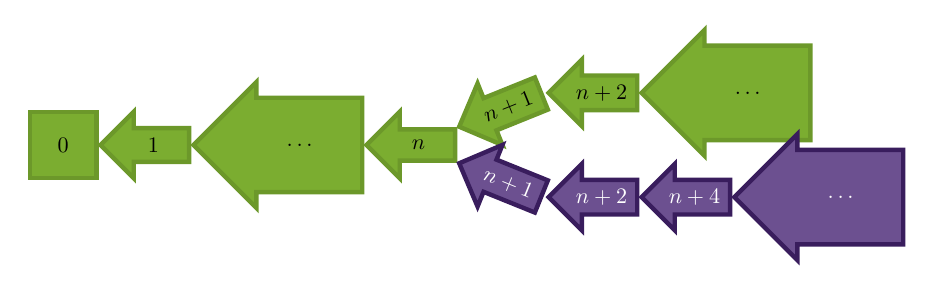
\begin{tikzpicture}[scale=0.8%, every node/.style={transform shape}
    , every node/.style={transform shape,XMRColor, ultra thick, shape border rotate = 180}
    , box/.style={minimum height = 30pt, minimum width = 30pt}
    , arr/.style={single arrow, minimum width = 30pt, minimum height = 40pt, anchor=tip}
    ]
\node[box] (last) at (-2,0){0};% top color=vir6, bottom color=vir8,
\node[arr] (last) at (last.east) {1};%\node[arr] (last) at (last.east) {2};
\node[arr, inner sep=20pt] (last) at (last.east) {\ldots};
\node[arr] (f1) at (last.east) {$n$};
% Fork 1 
\node[arr,rotate=22] (last) at (f1.before tail){$n+1$};
    \node[arr,xshift = 0.5mm] (last) at (last.east) {$n+2$};
    \node[arr, inner sep=20pt] (last) at (last.east) {\ldots};
% Fork 2
\node[arr, XMVColor, rotate = -22] (last) at (f1.after tail){$n+1$};
    \node[arr,XMVColor,xshift = 0.5mm] (last) at (last.east) {$n+2$};
    % \node[arr,XMVColor] (last) at (last.east) {$n+3$};
    \node[arr,XMVColor] (last) at (last.east) {$n+4$};
    \node[arr,XMVColor, inner sep=20pt] (last) at (last.east) {\ldots};
\end{tikzpicture}
		\end{center}
		\item Pre-fork funds can be spent on both chains
		\item This can be exploited for linking/tracing analysis
	\end{itemize}
\end{frame}

\begin{frame}{Cross Chain (Fork) Analysis}
\begin{itemize}[<+->]
	% \item Bitcoin \& Bitcoin Cash:
	% \begin{itemize}
	% 	\item Multiple Input Heuristic employed by GraphSense
	% 	\item If pre-fork funds are spent, addresses could be clustered on both post-fork branches
	% \end{itemize}
	% \item Monero:
	% \begin{itemize}
		\item Double spends are prevented with \emph{key images}
		\item Key image is derived from spent output and may occur at most once on the TX record
		\item Method to derive key image must be identical on all branches
		\item If two rings on two branches have the same key image, they spend the same TXO. 
	% \end{itemize}
\end{itemize}
\end{frame}

\subsection{Contribution of this work}
\begin{frame}{Contribution of this work}
	\begin{itemize}
		\item Up to date evaluation of existing methods
		\begin{itemize}
			\item Previous studies published shortly after introduction of RingCT
			\item Changes to mixin sampling and ringsize in 09/2017 and 04/2018.
		\end{itemize}
		\item Quantify impact on traceability from recent Monero hardforks \begin{itemize}
			\item Monero Original: Continuation of Monero v6 (ASIC compatible)
			\item MoneroV: Fork with some changes to emission curve
		\end{itemize}
	\end{itemize}
\end{frame}

\section{Results}
\subsection{Dataset}
\begin{frame}{Dataset \& Method}
	\begin{enumerate}
		\item Exported Monero (XMR), MoneroV (XMV) and Monero Original (XMO) blockchain up to Aug. 31$^\text{th}$, 2018.
		\item Employed Zero Mixin Removal \& Intersection Removal
		\item Added fork data and applied cross chain analysis (+ZMR/IR)
		\item Applied heuristics from \cite{kumar_traceability_2017} and \cite{moser_empirical_2018}:
		\begin{itemize}
			\item Guess Newest Heuristic
			\item Output Merging Heuristic
		\end{itemize}
		\item Evaluated accuracy with ground truth (where possible) with results from steps 3.
	\end{enumerate}
\end{frame}

\begin{frame}{Monero Activity}
	\def\imgFile{./img/slides/txs.tex}
	\resizebox{\textwidth}{!}{\input{\imgFile}}
\end{frame}
\subsection{Results}
\begin{frame}{Traced Inputs}
	\def\imgFile{./img/slides/linked.tex}
	\input{\imgFile}
\end{frame}
\begin{frame}
	\pgfplotstableread{./data/ringsizes/ringsizesNontrivial.csv}\ringsizes
	\def\rsCSV{https://git.io/flUOZ}
	\def\imgFile{./img/slides/rsp1.tex}
	\resizebox{\textwidth}{!}{\input{\imgFile}}
\end{frame}
\begin{frame}
	\pgfplotstableread{./data/ringsizes/ringsizesNontrivial.csv}\ringsizes
	\def\rsCSV{https://git.io/flUOZ}
	\def\imgFile{./img/slides/rsp2.tex}
	\resizebox{\textwidth}{!}{\input{\imgFile}}
\end{frame}


\begin{frame}{Guess Newest Heuristic}
	\def\imgFile{./img/slides/guess_newest.tex}
	\input{\imgFile}
\end{frame}
\begin{frame}{Output Merging Heuristic}
	\def\imgFile{./img/slides/merge_stats.tex}
	\input{\imgFile}
\end{frame}
\begin{frame}{Inputs/Outputs (per TX)}
	\def\imgFile{./img/slides/inputs.tex}
	\input{\imgFile}
\end{frame}


\begin{frame}{Summary}
	\begin{itemize}[<+->]
		\item Nowadays, most Monero TXs are untraceable
		\item Guess Newest Heuristic does not work with current mixin sampling technique
		\item Impact from Cross Chain Analysis not very large
		\begin{enumerate}
			\item Forks didn't have a lot of traction
			\item Mandatory ringsize of 7 enough to prevent chain reactions
		\end{enumerate}
	\end{itemize}
\end{frame}


\begin{frame}[allowframebreaks]{References}
    \bibliographystyle{apalike-refs}
    \bibliography{cryptoPoster}
\end{frame}

\subsection{Appendix}
\begin{frame}{Bitcoin analytics}
	\begin{itemize}
		\item Analysis techniques impeded privacy of Bitcoin
		\item Sets of addresses belonging to a user can often be identified 
		\begin{itemize}
			\item Multi Input Heuristic
			\item Change Heuristics
		\end{itemize}
		\item Simplified transaction graph allows further analysis
	\end{itemize}
\end{frame}

\begin{frame}{Multiple Input Heuristic (MIH)}\label{sec:mih}
	\resizebox{\textwidth}{!}{% !TeX root = ../../CI-Slides.tex
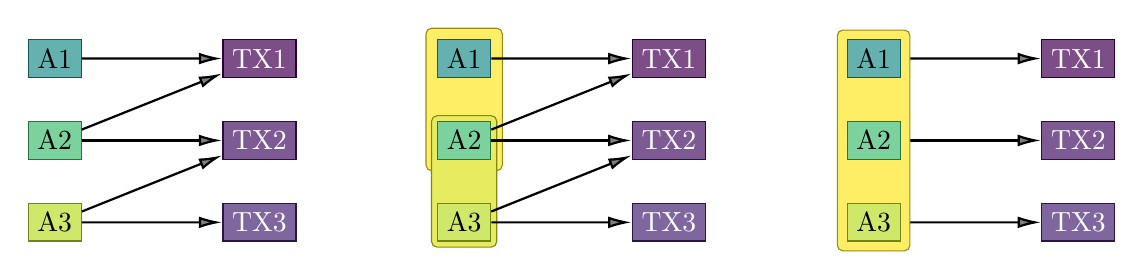
\begin{tikzpicture}[scale=1.3, -{Latex[length=3mm, width=1.5mm]}, deposit/.style={txColor, dashed}] 
\coordinate (C1) at (2,2);

\begin{scope}[xshift=-4.cm]
    \node[virNode=0.5] (X1) at (-1,0.8){A1}; 
    \node[virNode=0.7] (X2) at (-1,0){A2}; 
    \node[virNode=0.9] (X3) at (-1,-0.8){A3}; 
    \node[virNode=0.0,text=white] (Y1) at (1,0.8){TX1};
    \node[virNode=0.05,text=white] (Y2) at (1,0){TX2};
    \node[virNode=0.1,text=white] (Y3) at (1,-0.8){TX3};
   
    \path[thick, nodeBlack](X1) edge[] (Y1);
    \path[thick, nodeBlack](X2) edge[] (Y2);
    \path[thick, nodeBlack](X2) edge[] (Y1);
    \path[thick, nodeBlack](X3) edge[] (Y2);
    \path[thick, nodeBlack](X3) edge[] (Y3);
\end{scope}
\uncover<2->{
\begin{scope}[xshift=0.0cm]
    \node[virNode=0.5] (X1) at (-1,0.8){A1}; 
    \node[virNode=0.7] (X2) at (-1,0){A2}; 
    \node[virNode=0.9] (X3) at (-1,-0.8){A3}; 
    \node[virNode=0.0,text=white] (Y1) at (1,0.8){TX1};
    \node[virNode=0.05,text=white] (Y2) at (1,0){TX2};
    \node[virNode=0.1,text=white] (Y3) at (1,-0.8){TX3};
   
    \path[thick, nodeBlack](X1) edge[] (Y1);
    \path[thick, nodeBlack](X2) edge[] (Y2);
    \path[thick, nodeBlack](X2) edge[] (Y1);
    \path[thick, nodeBlack](X3) edge[] (Y2);
    \path[thick, nodeBlack](X3) edge[] (Y3);
    \begin{scope}[on background layer]
        \uncover<2->{
            \node[virNode=1.00,opacity=1.0,inner sep=4pt,fit={(X1) (X2)}, rounded corners=2pt ] (E1) {};
        }
        \uncover<3->{
            \node[virNode=0.95,opacity=1.0,inner sep=2pt,fit={(X2) (X3)}, rounded corners=2pt] (E2) {};
        }
    \end{scope}
\end{scope}}
\uncover<4->{
\begin{scope}[xshift=4.cm]
    \node[virNode=0.5] (X1) at (-1,0.8){A1}; 
    \node[virNode=0.7] (X2) at (-1,0){A2}; 
    \node[virNode=0.9] (X3) at (-1,-0.8){A3}; 
    \node[virNode=0.0,text=white] (Y1) at (1,0.8){TX1};
    \node[virNode=0.05,text=white] (Y2) at (1,0){TX2};
    \node[virNode=0.1,text=white] (Y3) at (1,-0.8){TX3};
    \begin{scope}[on background layer]
        \uncover<4->{
        \path[thick, nodeBlack](X1) edge[] (Y1);
        \path[thick, nodeBlack](X2) edge[] (Y2);
        \path[thick, nodeBlack](X3) edge[] (Y3);
        \node[virNode=1,fit={(X1) (X3)}, rounded corners=2pt] (E1) {};
        }
    \end{scope}
\end{scope}}

\end{tikzpicture} }
	\begin{itemize}[<+->] % <+-| alert@+>
 		\item Transactions TX1-TX3 spend outputs belonging to A1-A3
		\item All outputs spent in a TX likely belong to the same person
		\item Overlapping clusters are merged
		% \item Scala library: \href{https://github.com/graphsense/graphsense-clustering}{github.com/graphsense/graphsense-clustering}
		% \qrcode{https://github.com/graphsense/graphsense-clustering}
	\end{itemize}
	\footnotetext{Back: \ref{sec:monero}}
\end{frame}
\begin{frame}{Address Clustering}
	\resizebox{\textwidth}{!}{% !TeX root = ../../CI-Poster.tex
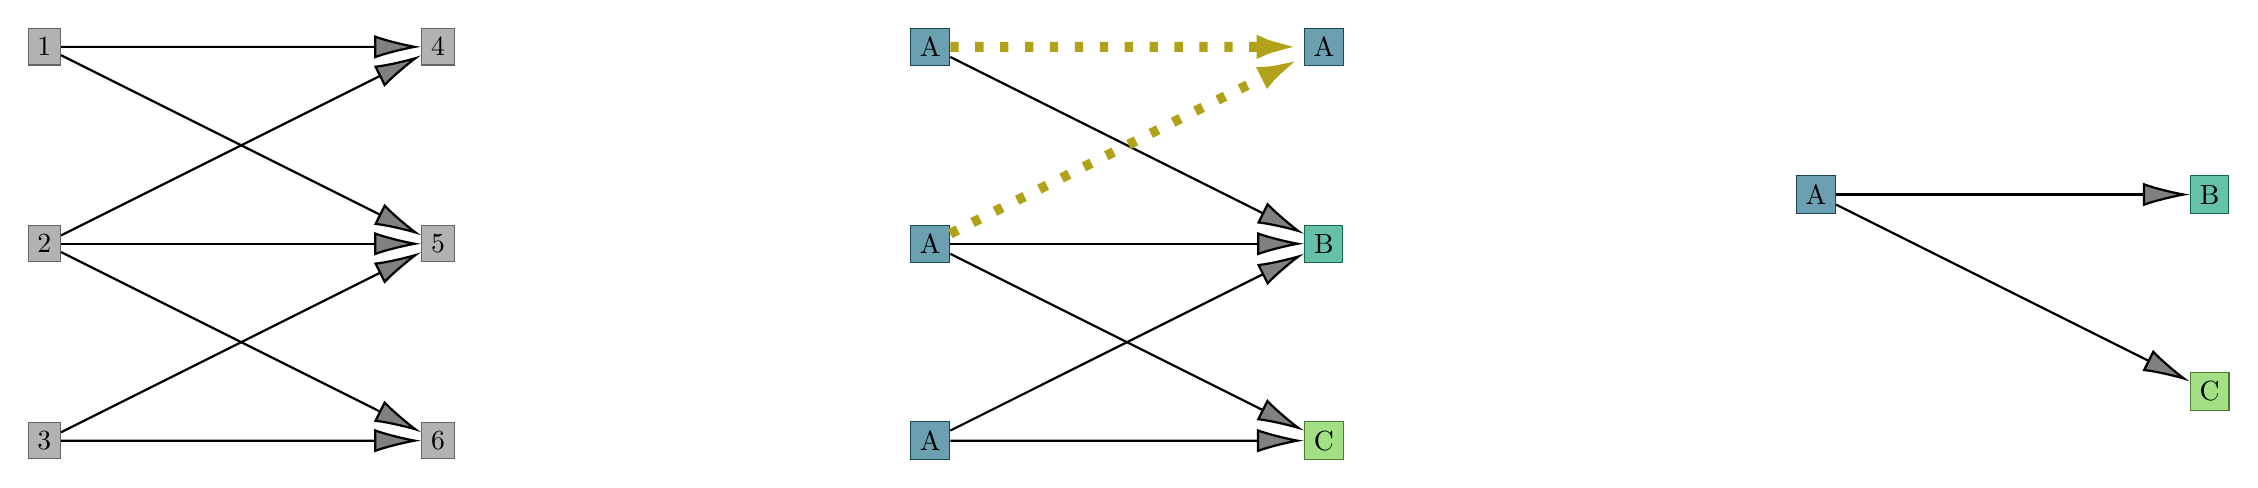
\begin{tikzpicture}[scale=2.5, -{Latex[length=6mm, width=3mm]}
    ,   remEdge/.style={line width=1.25mm, loosely dashed, virNodeDark=1.0} 
    ,   txNode/.style={opacity=1.0,inner sep=6pt,rounded corners=2pt}
    ,   sureEdge/.style={line width=1.25mm, virNodeDark=0.7}] 
\coordinate (C1) at (2,2);

\begin{scope}[xshift=-4.5cm]
    \node[nodeWhite] (X1) at (-1,1){1}; 
    \node[nodeWhite] (X2) at (-1,0){2}; 
    \node[nodeWhite] (X3) at (-1,-1){3}; 
    \node[nodeWhite] (Y1) at (1,1){4};
    \node[nodeWhite] (Y2) at (1,0){5};
    \node[nodeWhite] (Y3) at (1,-1){6};
    
    \path[thick, nodeBlack](X1) edge[] (Y1);
    \path[thick, nodeBlack](X2) edge[] (Y1);
    \path[thick, nodeBlack](X1) edge[] (Y2);
    \path[thick, nodeBlack](X2) edge[] (Y2);
    \path[thick, nodeBlack](X2) edge[] (Y3);
    \path[thick, nodeBlack](X3) edge[] (Y2);
    \path[thick, nodeBlack](X3) edge[] (Y3);
\end{scope}

\begin{scope}[]
    \node[virNode=0.4] (X1) at (-1,1){A}; 
    \node[virNode=0.4] (X2) at (-1,0){A}; 
    \node[virNode=0.4] (X3) at (-1,-1){A}; 
    \node[virNode=0.4] (Y1) at (1,1){A};
    \node[virNode=0.6] (Y2) at (1,0){B};
    \node[virNode=0.8] (Y3) at (1,-1){C};
   
    \path[thick, nodeBlack](X1) edge[] (Y2);
    \path[thick, nodeBlack](X2) edge[] (Y2);
    \path[thick, nodeBlack](X2) edge[] (Y3);
    \path[thick, nodeBlack](X3) edge[] (Y2);
    \path[thick, nodeBlack](X3) edge[] (Y3);
    \path[remEdge](X1) edge[] (Y1);
    \path[remEdge](X2) edge[] (Y1);
\end{scope}
\begin{scope}[xshift=4.5cm]
    \node[virNode=0.4] (X2) at (-1,0.25){A}; 
    
    \node[virNode=0.6] (Y2) at (1,0.25){B};
    \node[virNode=0.8] (Y3) at (1,-.75){C};
    
    \path[thick, nodeBlack](X2) edge[] (Y2);
    \path[thick, nodeBlack](X2) edge[] (Y3);
\end{scope}

\end{tikzpicture} }
	\begin{itemize}[<+->] % <+-| alert@+>
	\item Address graph shows addresses (1-6) and TXs (edges)
	\item Use information from e.g. MIH to label nodes
	\item Simplify graph: Address graph $\Rightarrow$ Entity graph
	\end{itemize}
	\footnotetext{Back: \ref{sec:monero}}
\end{frame}


% \subsection{Cross-Chain Traceability}
% \subsection{Accuracy OMH}
% \subsection{Accuracy GNH}
% \end{document}
\end{document}